\documentclass[11pt]{article}

\usepackage{nmrdoc}
\usepackage{siunitx}
\usepackage{bm}
\usepackage{tikz}

\sisetup{per-mode=symbol}
\DeclareSIUnit{\angstrom}{\text{\AA}}

\newcommand{\code}[1]{\texttt{#1}}
\setlength{\parindent}{0pt}
\setlength{\parskip}{0.42em}
\emergencystretch=2em

\begin{document}
\NmrTitle{Numerical Addendum: Haigh--Mallion Calculator}

Strip the physics away and the calculator is one integral and the work that surrounds
it. The integral sums a dipole-shaped field over the flat interior of an aromatic ring,
cheaply where the integrand is smooth and carefully where the target nucleus comes close
enough to make it spike; getting that one integral right is most of the job. The
surrounding work reconstructs the ring's surface so there is something to integrate over,
contracts the result onto the ring's axis, and folds it into the tensor form the rest of
the library uses. The listings below are distilled from the source --- loops and
bookkeeping trimmed --- but the constants, guards, and arithmetic are the
implementation's. A glossary at the end defines the recurring terms.

\section{Reconstructing the ring}

Before anything can be integrated there has to be a surface to integrate over, and an
axis to project the result onto later. The surface is the ring's own interior, taken as
it sits --- buckled and all. The axis is the ring normal, and because thermal motion
bends an otherwise flat ring, that normal is not given; it is fit.

The straightforward pieces first. \code{RingTopology} gives each ring its vertices in a fixed cyclic
order --- a canonical chemistry walk (ipso, ortho, meta, para, and so on), not a sort by
geometric angle. That order is used later: the first three vertices fix the sign of the
normal. The centre \(\bm c\) is their mean.

\begin{codebox}
// Vertex orders, distilled from RingTopology.cpp.
PHE_or_TYR = {Ipso, Ortho1, Meta1, Para, Meta2, Ortho2};
HIS        = {Ipso, DeltaN, PyrroleAlpha, EpsilonN, PyrroleBeta};
TRP6       = {BridgeToOrtho1, BridgeToOrtho2, Ortho2, Meta2, Meta1, Ortho1};
\end{codebox}

The normal is a total-least-squares plane fit, done by SVD. We have five to nine atoms
lying close to a common plane and we want the normal of that plane. The normal is the
direction in which the atoms vary \emph{least} --- they spread out within the plane and
barely at all across it. A singular value decomposition of the centred coordinates ranks
the three axes by that spread, and the right singular vector with the smallest singular
value is the normal. A plane has two normals and the SVD does not single out one, so a
cross product of the first two edges sets the sign. A three-point cross product alone
would read the buckle of whichever three atoms it picked as the tilt of the whole ring;
the fit reads all of them.

\begin{codebox}
geo.center = mean(geo.vertices);

// Best-fit plane: SVD of the centered N x 3 coordinates.
Eigen::MatrixXd coords(geo.vertices.size(), 3);
for (size_t i = 0; i < geo.vertices.size(); ++i)
    coords.row(i) = (geo.vertices[i] - geo.center).transpose();

Eigen::JacobiSVD<Eigen::MatrixXd> svd(coords, Eigen::ComputeFullV);
geo.normal = svd.matrixV().col(2);    // smallest singular value = least spread

// A plane has two normals; pick the sign with the first two edges.
Vec3 e1 = geo.vertices[1] - geo.vertices[0];
Vec3 e2 = geo.vertices[2] - geo.vertices[0];
if (geo.normal.dot(e1.cross(e2)) < 0) geo.normal = -geo.normal;
\end{codebox}

The radius the filters later use is the \emph{mean} centre-to-vertex distance, not the
largest, so one atom lifted out of plane does not set the radius by itself.

The surface to integrate over is that same interior, fanned into triangles from the mean
centre out to the actual vertices --- piecewise planar through the buckled positions,
never flattened onto the fitted plane. The ring is convex, so the fan tiles it with no
mesher; a five-, six-, or nine-membered ring gives five, six, or nine triangles (the
nine-membered ring is the tryptophan indole perimeter).

\begin{codebox}
for (int i = 0; i < n; ++i) {                 // n = vertex count
    int j = (i + 1) % n;                       // wrap last vertex to first
    AccumulateAdaptiveTriangleIntegral(geom.center, verts[i], verts[j],
                                       point, qpts, H, /*level=*/0);
}
\end{codebox}

\section{Integrating over the face}

Now the integral itself. Over each triangle the code integrates the dipolar kernel ---
the field shape of a point magnet --- between the surface and the target atom. Far from
the ring that integrand is smooth and a few samples capture it; up close it climbs toward
the \(1/\rho^3\) pole, where a fixed handful of samples would miss the spike. The method
meets both cases with one idea: a fixed rule on each triangle, and more triangles where
the atom is near.

The fixed rule is a seven-point symmetric cubature, exact for polynomials up to degree
five: seven samples whose weighted average reproduces the integral of any quintic
exactly, so a smooth integrand costs little. The seven points are the triangle's
centroid, three near the vertices, and three near the edge midpoints, with weights built
from \(\sqrt{15}\); the weights sum to one, so the triangle's area \(A_T\) multiplies in
once, on its own. A sample's position is read in barycentric coordinates --- three weights
saying how much to lean on each corner.

\begin{codebox}
double root = std::sqrt(15.0);
double a1 = (6.0 - root) / 21.0,     a2 = (6.0 + root) / 21.0;
double w0 = 9.0 / 40.0;
double w1 = (155.0 - root) / 1200.0, w2 = (155.0 + root) / 1200.0;

pts = {{ {{1./3, 1./3, 1./3}, w0},                  // centroid
         {{a1, a1, 1-2*a1}, w1}, /* + 2 perms */     // three near vertices
         {{a2, a2, 1-2*a2}, w2}, /* + 2 perms */ }}; // three near midpoints
\end{codebox}

At each sample the code forms \code{sep}, the separation \(\bm\rho = \bm r - \bm s\) from
the surface point \(\bm s\) to the field point \(\bm r\), and adds the dipolar tensor to
all nine entries of \(\bm H\):
\[
  A_T\,w_q\left(\frac{3\rho_a\rho_b}{\rho^5} - \frac{\delta_{ab}}{\rho^3}\right).
\]
Two guards gate that sum. The singularity guard skips any sample within
\SI{0.1}{\angstrom} of the field point: the pole is real, not a rounding artefact, so the
code drops the samples it cannot evaluate. The area guard drops a triangle thinner than
\(10^{-20}\,\si{\angstrom^2}\) before it is ever sampled. Both are hard omissions --- the
skipped terms leave the sum, and nothing is reweighted to make up for them.

\begin{codebox}
double area = 0.5 * (v1 - v0).cross(v2 - v0).norm();
if (area < cfg("haigh_mallion_triangle_area_guard")) return;   // degenerate sliver

Vec3 s   = qp.lambda[0]*v0 + qp.lambda[1]*v1 + qp.lambda[2]*v2; // surface point
Vec3 sep = field_point - s;
double rho = sep.norm();
if (rho < cfg("singularity_guard_distance")) continue;         // step around the pole

double rho3 = rho*rho*rho, rho5 = rho3*rho*rho;
H(a,b) += qp.weight * area *
          (3.0*sep(a)*sep(b)/rho5 - (a==b ? 1.0 : 0.0)/rho3);
\end{codebox}

The indices \(a,b\) run over
\(x,y,z\). The adaptive part is a heuristic, not an error estimate. A triangle splits when
the target atom is within \SI{2.0}{\angstrom} of any of its vertices at the top level,
\SI{1.0}{\angstrom} one level down; a split swaps it for four midpoint subtriangles, and
the recursion stops at depth two. So one fan triangle costs seven samples when the atom is
far, twenty-eight after a split, and at most \(16\times7 = 112\) when every subtriangle
splits in turn --- across a whole ring, at most 560, 672, or 1008 samples. Refinement
concentrates the samples where the atom is close, and the depth-two cap bounds the cost:
112 per triangle, whatever the geometry.

\begin{codebox}
bool subdivide = false;
if      (level == 0) subdivide = near_vertex(field_point, v0, v1, v2,
                                    cfg("haigh_mallion_subdivision_threshold_l1"));
else if (level == 1) subdivide = near_vertex(field_point, v0, v1, v2,
                                    cfg("haigh_mallion_subdivision_threshold_l2"));
if (subdivide) {                       // false at level 2, so it stops
    Vec3 m01 = 0.5*(v0+v1), m12 = 0.5*(v1+v2), m02 = 0.5*(v0+v2);
    recurse(v0,  m01, m02, level+1);   recurse(m01, v1,  m12, level+1);
    recurse(m02, m12, v2,  level+1);   recurse(m01, m12, m02, level+1);
} else {
    AccumulateTriangleIntegral(v0, v1, v2, field_point, qpts, H);
}
\end{codebox}

\begin{figure}[ht]
\centering
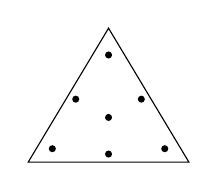
\begin{tikzpicture}[scale=0.85,line width=0.4pt]
  \coordinate (A) at (0,0);
  \coordinate (B) at (2.4,0);
  \coordinate (C) at (1.2,2.0);
  \draw (A) -- (B) -- (C) -- cycle;
  \fill (1.2,0.667) circle (1.5pt);
  \fill (0.36,0.20) circle (1.5pt);
  \fill (2.04,0.20) circle (1.5pt);
  \fill (1.2,1.60) circle (1.5pt);
  \fill (1.2,0.12) circle (1.5pt);
  \fill (1.69,0.94) circle (1.5pt);
  \fill (0.71,0.94) circle (1.5pt);
\end{tikzpicture}
\hspace{2.5em}
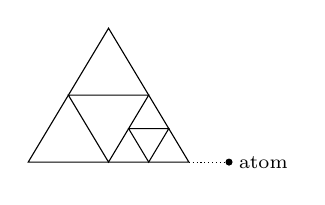
\begin{tikzpicture}[scale=0.85,line width=0.4pt]
  \coordinate (A) at (0,0);
  \coordinate (B) at (2.4,0);
  \coordinate (C) at (1.2,2.0);
  \coordinate (mAB) at (1.2,0);
  \coordinate (mBC) at (1.8,1.0);
  \coordinate (mAC) at (0.6,1.0);
  \draw (A) -- (B) -- (C) -- cycle;
  \draw (mAB) -- (mBC) -- (mAC) -- cycle;
  \draw (1.8,0) -- (2.1,0.5) -- (1.5,0.5) -- cycle;
  \draw[densely dotted] (B) -- (3.0,0);
  \fill (3.0,0) circle (1.5pt) node[right] {\scriptsize atom};
\end{tikzpicture}
\caption{The seven-point rule on a fan triangle (left). When the target atom is near,
the triangle splits at its edge midpoints, and the subtriangle nearest the atom splits
again (right), so the triangles --- each carrying the rule shown on the left ---
concentrate where the atom is close.}
\end{figure}

By the time any of this runs the atom--ring pair has already cleared a spatial query
--- ring centres within \SI{15}{\angstrom} --- and three filters: one rejecting
near-coincident centres, a near-field one rejecting separations not greater than the ring radius
(\code{source\_extent} is twice \code{geom.radius}), and a bonded-exclusion that drops the
ring's own atoms and their immediate neighbours.

\section{From the integral to the kernel}

The accumulated \(\bm H\) is a \(3\times3\) tensor that has folded in the whole ring's
geometry as seen from this atom. Turning it into the reported shielding kernel is one
contraction. The physics asks for the field along the ring's axis, so \(\bm H\) is
contracted with the normal to give the effective field \(\bm V = \bm H\bm n\), and the
kernel is the outer product \(G_{ab} = -V_a n_b\). Being an outer product of two vectors,
\(\bm G\) is rank at most one --- rank one unless \(\bm V = \bm 0\) --- and because
\(\bm V\) need not point along \(\bm n\), it need not be symmetric.

\begin{codebox}
Mat3 H = ComputeSurfaceIntegralH(atom_pos, geom);
Vec3 V = H * geom.normal;                 // effective field, V = H n
Mat3 G;
for (int a = 0; a < 3; ++a)
    for (int b = 0; b < 3; ++b)
        G(a,b) = -geom.normal(b) * V(a);  // outer product -V n^T, rank 1

rn->hm_H_spherical = SphericalTensor::Decompose(H);
rn->hm_G_spherical = SphericalTensor::Decompose(G);
G_total += G;
\end{codebox}

One wrinkle: every sample added to \(\bm H\) is symmetric and traceless, so the exact
integral is too --- it is pure \(T_2\). The code does not re-impose that after the
floating-point sum, so a faint \(T_0\) or \(T_1\) residue can survive in
\code{hm\_H\_spherical}, left as the arithmetic produced it.

\section{The shared tensor projection}

Every tensor the calculator emits passes through \code{SphericalTensor::Decompose}, the
library's single move for splitting a \(3\times3\) tensor into the three pieces that
rotation shuffles within but never between: a scalar \(T_0\), a vector \(T_1\), and a
five-component shape \(T_2\). It is closed-form arithmetic, not an eigenproblem --- the
trace gives \(T_0\), the antisymmetric part gives \(T_1\), and the symmetric traceless
part gives \(T_2\).

\begin{codebox}
st.T0 = sigma.trace() / 3.0;                       // scalar

st.T1[0] = 0.5*(sigma(1,2) - sigma(2,1));          // antisymmetric part -> vector
st.T1[1] = 0.5*(sigma(2,0) - sigma(0,2));
st.T1[2] = 0.5*(sigma(0,1) - sigma(1,0));

double Sxx = sigma(0,0)-st.T0, Syy = sigma(1,1)-st.T0, Szz = sigma(2,2)-st.T0;
double Sxy = 0.5*(sigma(0,1)+sigma(1,0));          // symmetric traceless S
double Sxz = 0.5*(sigma(0,2)+sigma(2,0));
double Syz = 0.5*(sigma(1,2)+sigma(2,1));

st.T2[0] = std::sqrt(2.0)*Sxy;     st.T2[1] = std::sqrt(2.0)*Syz;
st.T2[2] = std::sqrt(3.0/2.0)*Szz;
st.T2[3] = std::sqrt(2.0)*Sxz;     st.T2[4] = (Sxx - Syy)/std::sqrt(2.0);
\end{codebox}

The factors on the five \(T_2\) entries are not decoration --- they make the packing
\emph{isometric}, so the length of the five-vector equals the Frobenius length of the
symmetric traceless matrix \(\bm S\) it came from. The \(\sqrt2\) on each off-diagonal
pays for double counting: \(S_{xy}\) sits in the matrix twice, as \(S_{xy}\) and
\(S_{yx}\), so it owes \(2S_{xy}^2\) to the Frobenius sum, and \(\sqrt2\,S_{xy}\) squares
to exactly that. The diagonal has only two free numbers once the trace is zero, and
\(\sqrt{3/2}\,S_{zz}\) with \((S_{xx}-S_{yy})/\sqrt2\) carry them so their squares add
back to \(S_{xx}^2+S_{yy}^2+S_{zz}^2\). So a dot product of two stored five-vectors is the
Frobenius inner product of the tensors they encode --- the similarity the calibration
uses, at five multiplies instead of nine.

For this calculator \(\bm H\) lands almost entirely in \(T_2\) by construction, while the
rank-one \(\bm G\) --- the reported kernel --- can carry all three channels.

\section{Glossary}

\textbf{Spherical (irreducible) tensor decomposition, \(T_0/T_1/T_2\).} Any \(3\times3\)
tensor splits into three parts that rotations never mix into one another: a single
number, an arrow, and a five-number ``shape'' that stretches along some directions and
shrinks along others. For a magnetic shielding tensor, \(T_0\) is the isotropic shielding that survives the
molecule's tumbling and \(T_2\) is the orientation-dependent anisotropy; the chemical
shift comes only after referencing and a sign convention.
Formally, the reducible representation \(\mathbf 3\otimes\mathbf 3\) of
\(\mathrm{SO}(3)\) decomposes into irreducibles of dimension \(1\), \(3\), and \(5\) ---
a scalar (the trace), a pseudovector (the antisymmetric part), and a symmetric traceless
tensor.

\textbf{Frobenius norm.} A matrix's overall size, blind to which way it points: string
its entries into one long vector and take that vector's length. The \(3\times3\) identity
has Frobenius norm \(\sqrt3\). Formally,
\(\|A\|_F = \big(\sum_{ij}A_{ij}^2\big)^{1/2} = (\operatorname{tr}A^{\mathsf T}A)^{1/2}\),
the norm of the trace inner product \(\langle A,B\rangle = \operatorname{tr}A^{\mathsf T}B\).

\textbf{Dipolar kernel.} The field shape of a small bar magnet --- strongest and signed
along its axis, weaker and reversed to the side, fading as the cube of distance. Along
the axis it is \(+2/\rho^3\), broadside \(-1/\rho^3\), and zero at the magic angle
(\(\ang{54.7}\)) where the two balance. Formally, it is the Hessian of \(1/\rho\), the
symmetric traceless tensor \((3\rho_a\rho_b - \delta_{ab}\rho^2)/\rho^5\).

\textbf{Barycentric coordinates.} A point inside a triangle named by how hard it leans on
each corner --- three weights that add to one. The centroid is
\((\tfrac13,\tfrac13,\tfrac13)\), the corner \(\bm v_0\) is \((1,0,0)\), and the midpoint
of \(\bm v_0\bm v_1\) is \((\tfrac12,\tfrac12,0)\). Formally,
\((\lambda_0,\lambda_1,\lambda_2)\) with \(\sum_i\lambda_i = 1\) and \(\lambda_i\ge 0\)
inside denote the point \(\lambda_0\bm v_0 + \lambda_1\bm v_1 + \lambda_2\bm v_2\).

\textbf{Total-least-squares plane fit (by SVD).} The best plane through a cloud of
nearly-coplanar points is the one they stray from least, and its normal is the lone
direction along which they barely spread. Were the points exactly coplanar, that spread
--- and the smallest singular value --- would be zero. Formally, the normal minimises
\(\sum_i\big(\bm n^{\mathsf T}(\bm x_i-\bm c)\big)^2\) over unit \(\bm n\), and is the
right singular vector of the mean-centred coordinates with the smallest singular value.

\textbf{Gauss cubature; degree of exactness.} A short stand-in for an integral over the
triangle: read the integrand at a few fixed points and take a weighted sum, which is the
exact integral for any low-degree polynomial. The seven-point rule here is exact for any
integrand up to a quintic; beyond degree five it is not guaranteed. Formally, a rule has
degree of exactness \(d\) when its weighted sum equals the integral for every polynomial
of total degree \(\le d\); here \(d = 5\).

\end{document}
